\documentclass[english, 11pt]{article}

\usepackage[T1]{fontenc}    % Riktig fontencoding
\usepackage[utf8]{inputenc} % Riktig tegnsett
\usepackage{babel}          % Ordelingsregler, osv
\usepackage{graphicx}       % Inkludere bilder
\usepackage{booktabs}       % Ordentlige tabeller
\usepackage{url}            % Skrive url-er
\usepackage{textcomp}       % Den greske bokstaven micro i text-mode
\usepackage{units}          % Skrive enheter riktig
\usepackage{float}          % Figurer dukker opp der du ber om
\usepackage{lipsum}         % Blindtekst
\usepackage{amsmath}        % Mattestæsj
\usepackage{listingsutf8}   % Kodetekst
\usepackage{verbatim}
\usepackage{subfigure}		% Flere fig. ved siden av hverandre
\usepackage[a4paper,margin=1.2in]{geometry}

\lstset{breaklines=True,numbers=left}

% JF i margen
\makeatletter
\renewcommand{\subsubsection}{\@startsection{subsubsection}{3}{-2cm}%
{-\baselineskip}{0.5\baselineskip}{\bf\large}}
\makeatother
\newcommand{\jf}[1]{\subsubsection*{JF #1}\vspace*{-2\baselineskip}}

% Skru av seksjonsnummerering
\setcounter{secnumdepth}{-1}

%, trim = 1cm 7cm 1cm 7cm % PDF-filer som bilde

\begin{document}

% Forside
\begin{titlepage}
\begin{center}

\textsc{\Large FYS4150 - Computational Physics}\\[0.5cm]
\rule{\linewidth}{0.5mm} \\[0.4cm]
{ \huge \bfseries  PROJECT 1}\\[0.10cm]
\rule{\linewidth}{0.5mm} \\[1.5cm]
\textsc{\Large svc}\\[1.5cm]
\textsc{}\\[1.5cm]

% Av hvem?
\begin{minipage}{0.49\textwidth}
    \begin{center} \large
        Henrik Sverre Limseth\\ \url{henrisli@uio.no} \\[0.8cm]
    \end{center}
\end{minipage}
\bigskip \\
\begin{minipage}{0.49\textwidth}
    \begin{center} \large
        Jon Vegard Sparre\\ \url{jonvsp@uio.no} \\[0.8cm]
    \end{center}
\end{minipage}
\begin{minipage}{0.49\textwidth}
    \begin{center} \large
        Anne-Marthe Hovda\\ \url{annemmho@uio.no} \\[0.8cm]
    \end{center}
\end{minipage}

\vfill

% Dato nederst
\large{Dato: \today}

\end{center}
\end{titlepage}

\abstract{}

\section*{Exercise a)}

\paragraph{Rewriting of differential equation}
We'll show that we can write our differential equation $-u''(x) = f(x)$ as the matrix equation $ Av = \tilde b$. First we use the three point formula for a second derivative to get

$$ -\frac{v_{i+1} + v_{i-1} - 2v_i}{h^2} = f_i, \quad \text{for } i=0,\ldots,n, $$

where we multiply both sides by $h^2$ such that we get $ \tilde b_i = h^2 f_i$. Then we simply write the matrix $A$ given in the exercise text and multiply it by $v$ to see what we get

\begin{align*}
	Av &=
	\left(\begin{matrix}
		2 & -1 & 0 & 0 &\ldots & 0 \\	
		-1 & 2 & -1 & 0 & \ldots & 0 \\
		0 & \ddots & \ddots & \ddots & \ddots & \vdots \\
		\vdots & \ddots & \ddots & \ddots & \ddots & 0 \\
		\vdots & \ddots & \ddots & \ddots & \ddots & -1 \\
		0 & \ldots & \ldots & 0 & -1 & 2 \\
	\end{matrix}\right)\left(
	\begin{matrix}
		v_1 \\ \vdots\\ \vdots \\ \vdots \\ \vdots \\ \vdots \\ v_n 
	\end{matrix} \right) \\
	&= \left(\begin{matrix}
		2v_1 & -v_2 & 0 & 0 &\ldots & 0 \\	
		-v_1 & 2v_2 & -v_3 & 0 & \ldots & 0 \\
		0 & \ddots & \ddots & \ddots & \ddots & \vdots \\
		\vdots & \ddots & \ddots & \ddots & \ddots & 0 \\
		\vdots & \ddots & \ddots & \ddots & \ddots & -v_n \\
		0 & \ldots & \ldots & 0 & -v_{n-1} & 2v_n \\
	\end{matrix}\right),
\end{align*}

where we recognize each row as the three point formula for the $i$-th component of $v$, \emph{e.g.} for $i=2$ we have

$$ -v_1 + 2v_2 -v_3 = \tilde b_2.$$

\paragraph{Checking the given solution}
We're given the source term $f(x) = 100 e^{-10x}$, and we'll check if the solution $u(x) = 1-(1-e^{-10})x - e^{-10x}$ is correct when we have the given $f(x)$ as a source term, by inserting it into to Poisson's equation.

\begin{align*}
	u(x) &= 1-(1-e^{-10})x - e^{-10x} \\
	u'(x) &= (1-e^{-10}) + 10e^{-10x} \\
	u''(x) &= - 100e^{-10x} = -f(x).
\end{align*}

\section*{Exercise b)}

The matrix $\mathbf A$ is rewritten as three column vectors in order to optimize our code. We then get $n$ equations,
$$ a_i v_{i-1} + b_iv_i + c_i v_{i+1} = \tilde b_i.$$
To solve this we do a forward and then a backward substitution. We do the forward substitution in order to get each $v_i$

\begin{align*}
	a_i v_{i-1} + b_iv_i + c_i v_{i+1} =  \tilde b_i \\
	v_i = \frac{\tilde b_i - a_i v_{i-1} - c_i v_{i+1}}{b_i} 
\end{align*}

For $i=0$ and $i=n$ we have the initial conditions, which are $u(0) = u(1)=0$. This implies that our matrix with all the $x$-values must have $n+2$ elements in our code since we have to add the end points manually.

For $i=1$ we get

\begin{align*}
	v_2 =  \frac{\tilde b_1 - a_1 v_0 - b_1v_1}{c_1} 
\end{align*}

\begin{align*}
	v_2 = \frac{\tilde b_2 - a_2 v_1 - c_2 v_{2}}{b_2} 
\end{align*}

Our algorithm is given below

\begin{lstlisting}
Declaring variables
...
Setting initial conditions
...

Make for loops that calculate v_i
for( i up to n) {
        temp[i] = c[i-1]/btemp;
        btemp = b[i]-a[i]*temp[i];
        v[i] = (f[i] - a[i]*v[i-1])/btemp;

Saving results

\end{lstlisting}

For our calculation we have $8n$ FLOPS, $6n$ in the first for-loop and then $2n$ more in the second for-loop.

\section*{Exercise c)} In this part of the project we did an analysis of the relative error between our own numerical solution and the exact solution. We calculated the error as described in the exercise text,
$$ \epsilon_i \log_{10} \left( \left| \frac{v_i - u_i}{u_i} \right|  \right). $$
In my program it looked like this.\\

\lstinputlisting[language=C++, firstline=108, lastline=119]{../main.cpp}

Below we see the table with our maximum relative errors. We see that it decreases when $n$ is increasing, remember that the error is written as the logarithm of the relative error. In fig. \ref{fig:en101}, \ref{fig:en102}, \ref{fig:en103}, \ref{fig:en104} and \ref{fig:en105} we see the errors plotted as a function of $x$. When $n=10$ the error is constant equal $-1.1797$, which must be a coincicence?

\begin{table}[H]
  \centering
  \begin{tabular}{ c c }
    \toprule
    $n$ & $\epsilon_{\text max}$ \\
    \midrule
	$10$ &	$-1.1797$ \\
	$10^2$ & $-3.0880$ \\
	$10^3$ & $-5.0800$ \\
	$10^4$ & $-7.0753$ \\
	$10^5$ & $-8.3667$ \\
    \bottomrule
  \end{tabular}
  \caption{Maximum error for different $n$ when using LU-decomposition with forward and backward substitution. At $n=10^6$ our program crashes. Also note that the error is decreasing with increasing $n$.}
  \label{tab:error_max}
\end{table}

\begin{figure}[H]
    \centering
    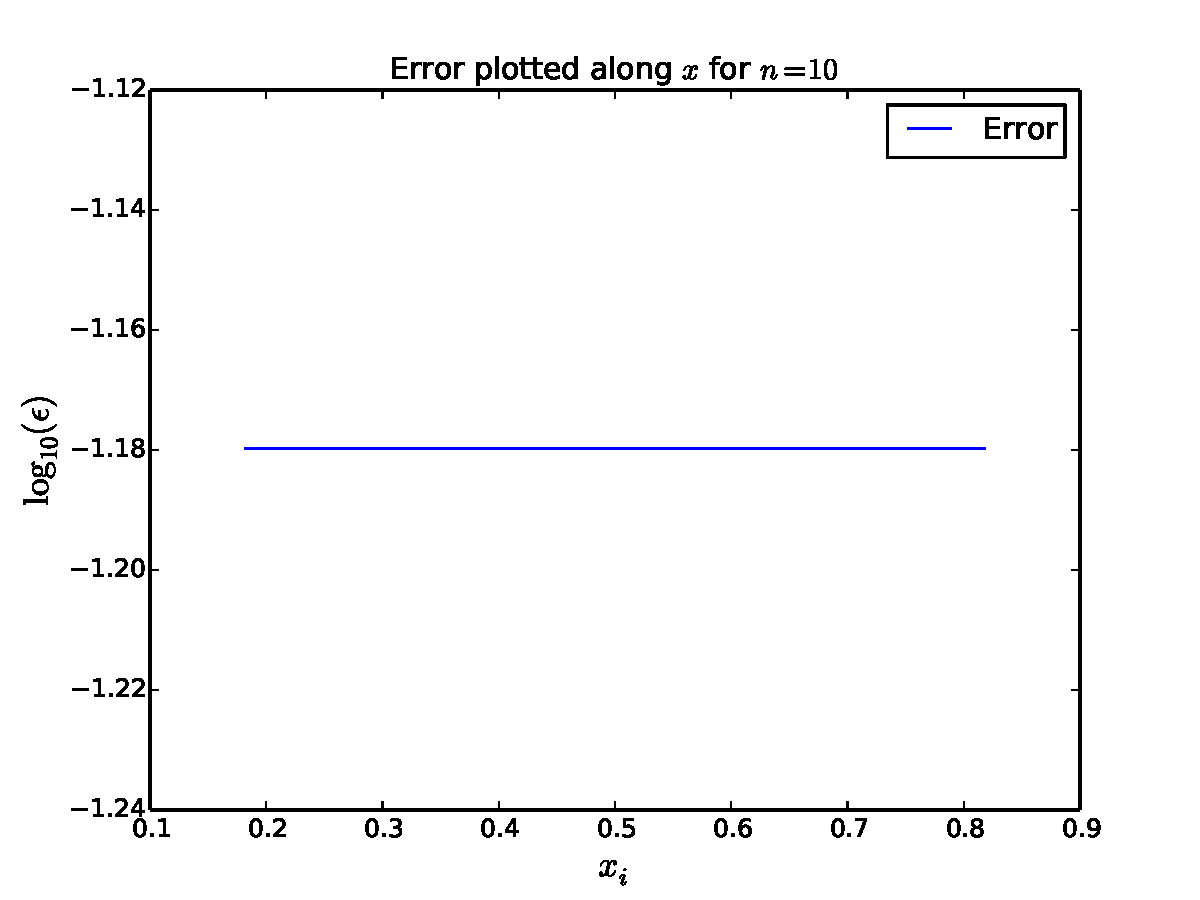
\includegraphics[width = .9\textwidth]{error_n_10.pdf}
    \caption{Error plot for $n=10$}
    \label{fig:en101}
\end{figure}

\begin{figure}[H]
    \centering
    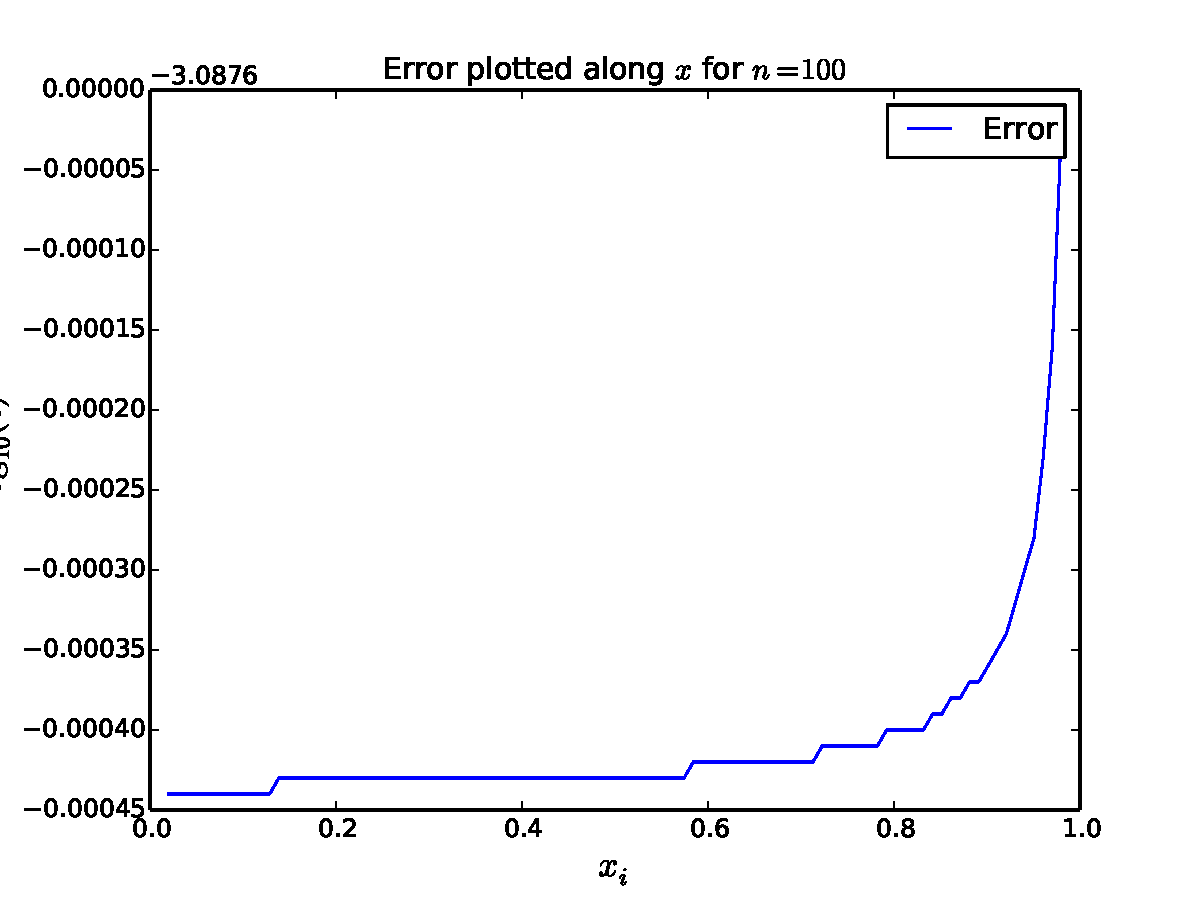
\includegraphics[width = \textwidth]{error_n_100.pdf}
    \caption{Error plot for $n=10^2$}
    \label{fig:en102}
\end{figure}

\begin{figure}[H]
    \centering
    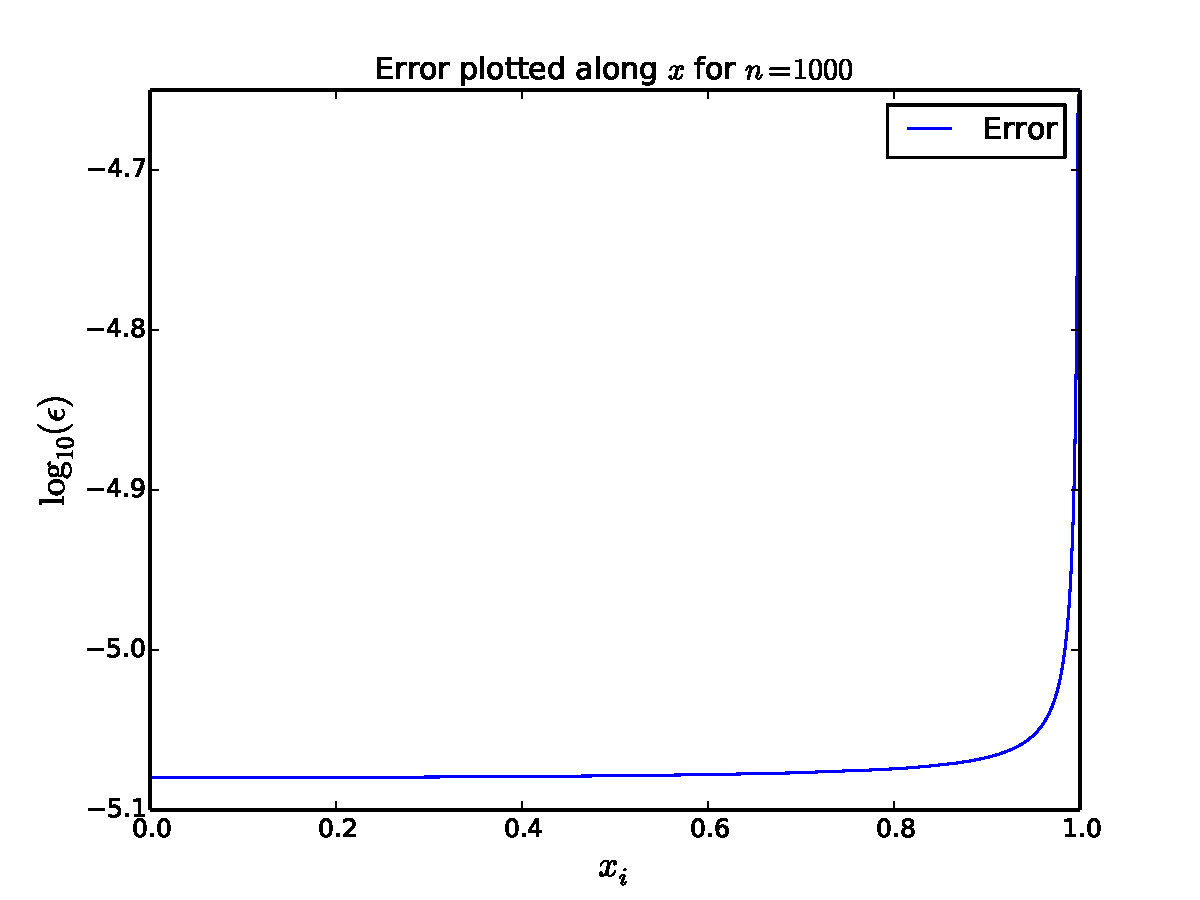
\includegraphics[width = .9\textwidth]{error_n_1000.pdf}
    \caption{Error plot for $n=10^3$}
    \label{fig:en103}
\end{figure}

\begin{figure}[H]
    \centering
    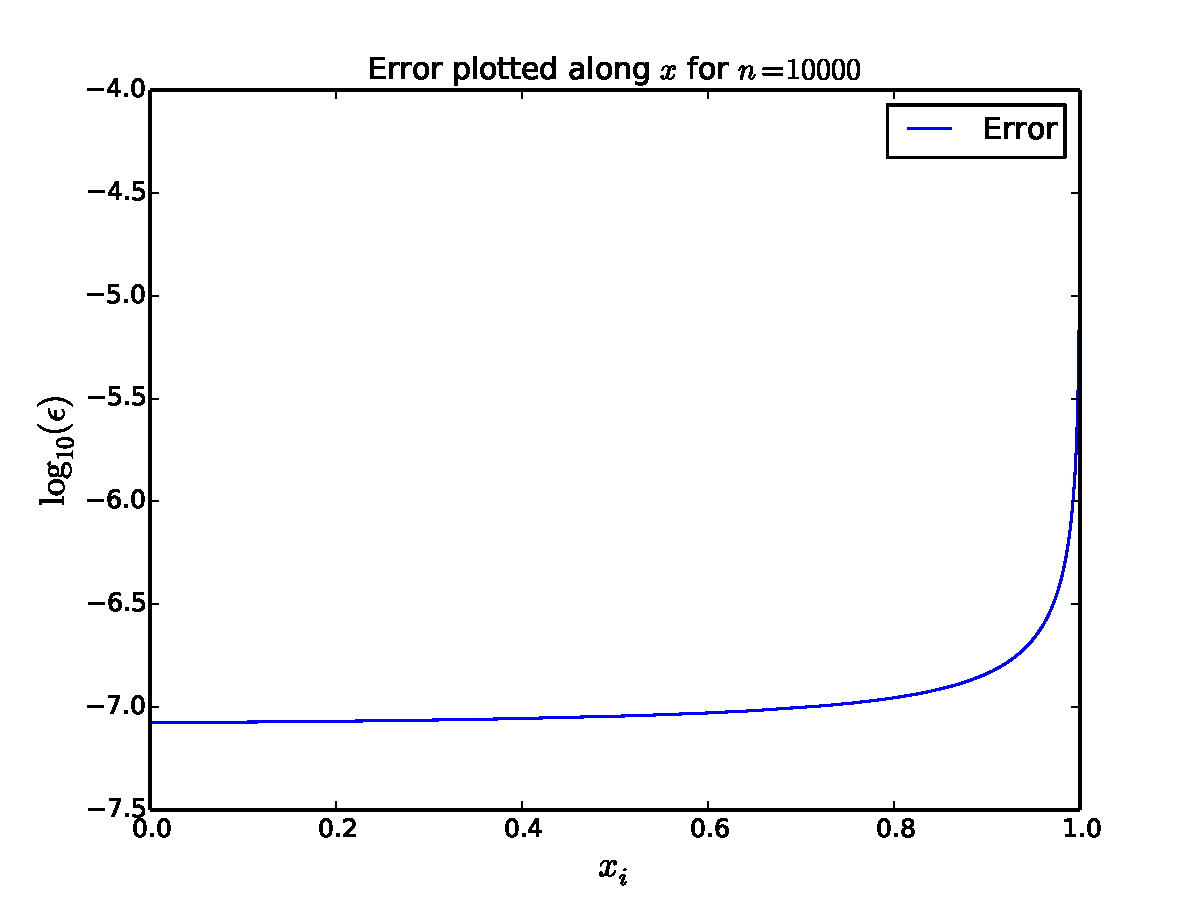
\includegraphics[width = .9\textwidth]{error_n_10000.pdf}
    \caption{Error plot for $n=10^4$}
    \label{fig:en104}
\end{figure}

\begin{figure}[H]
    \centering
    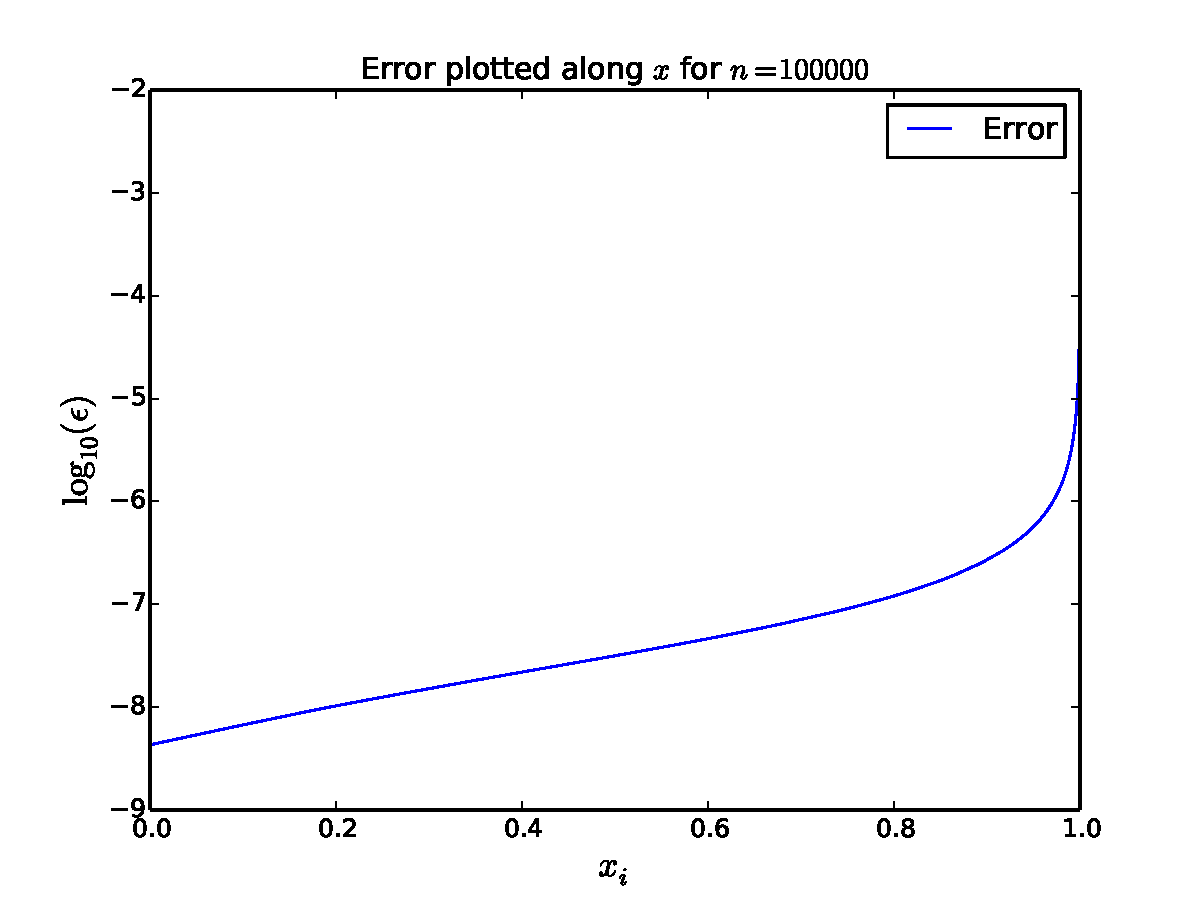
\includegraphics[width = .9\textwidth]{error_n_100000.pdf}
    \caption{Error plot for $n=10^5$}
    \label{fig:en105}
\end{figure}

\section*{Exercise d)} In this last part we're asked to compare our numerical results with the ones we get by using packages like Armadillo.

\begin{figure}[H]
    \centering
    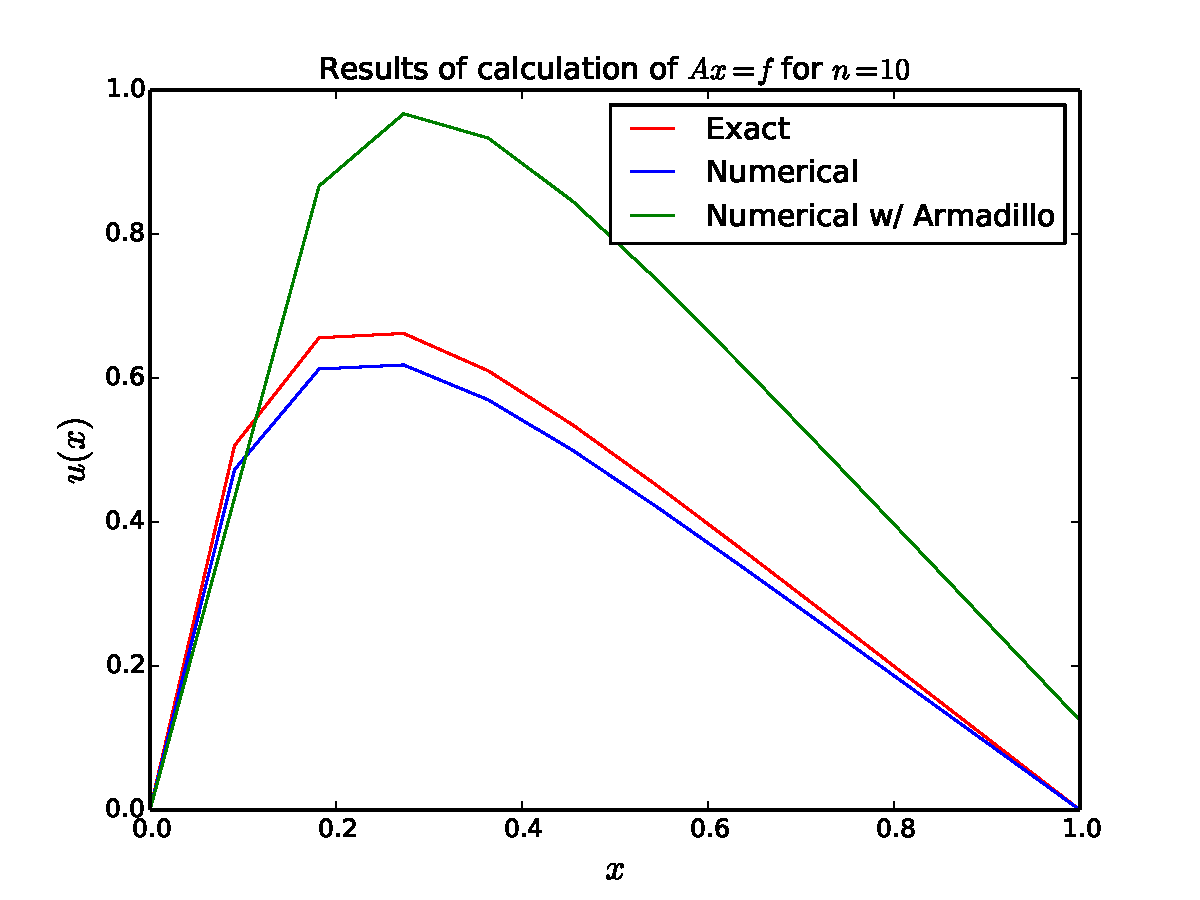
\includegraphics[width = .9\textwidth]{d_n_10.pdf}
    \caption{Numerical solution for $n=10^5$. Armadillo's function `solve' is pretty far off from the exact and the first numerical solution.}
    \label{fig:sol101}
\end{figure}

\begin{figure}[H]
    \centering
    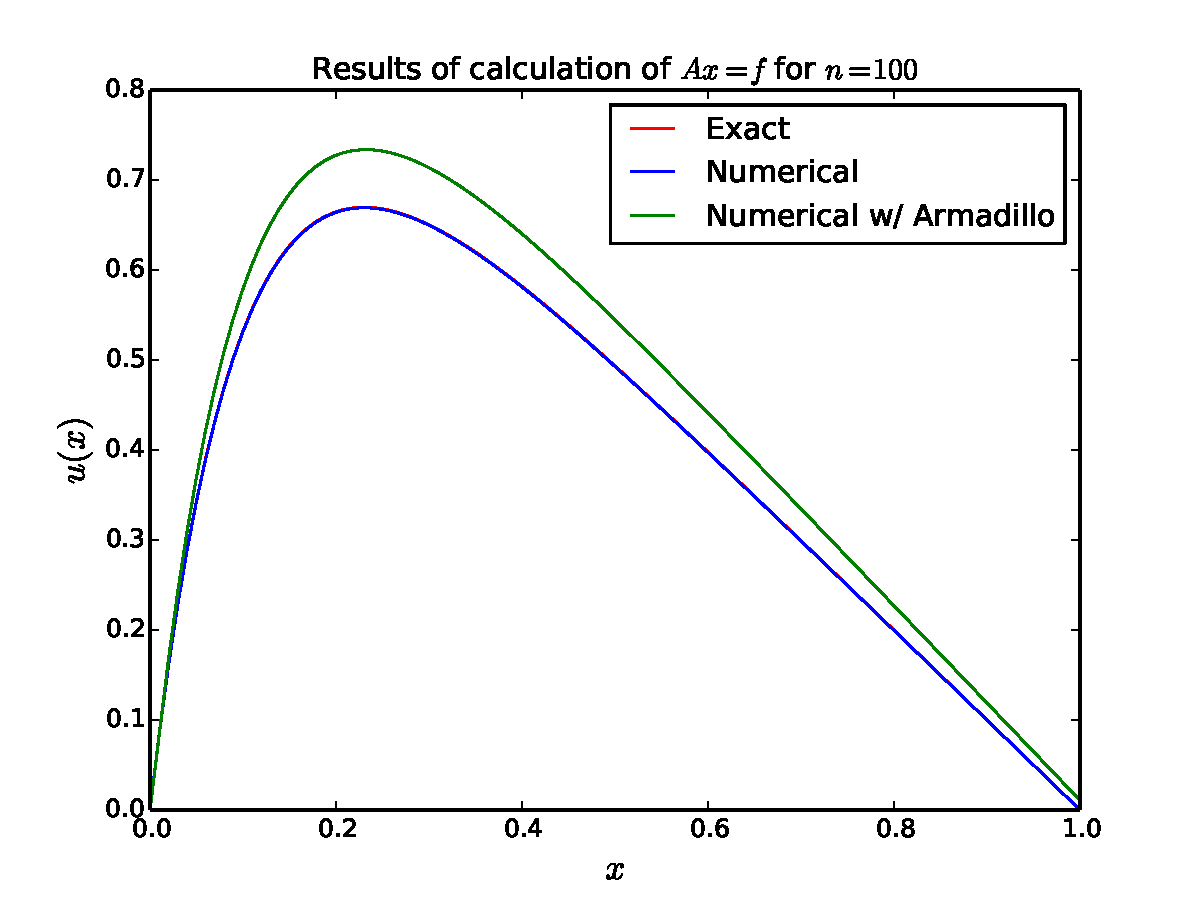
\includegraphics[width = .9\textwidth]{d_n_100.pdf}
    \caption{Numerical solution for $n=10^5$.}
    \label{fig:sol102}
\end{figure}

\begin{figure}[H]
    \centering
    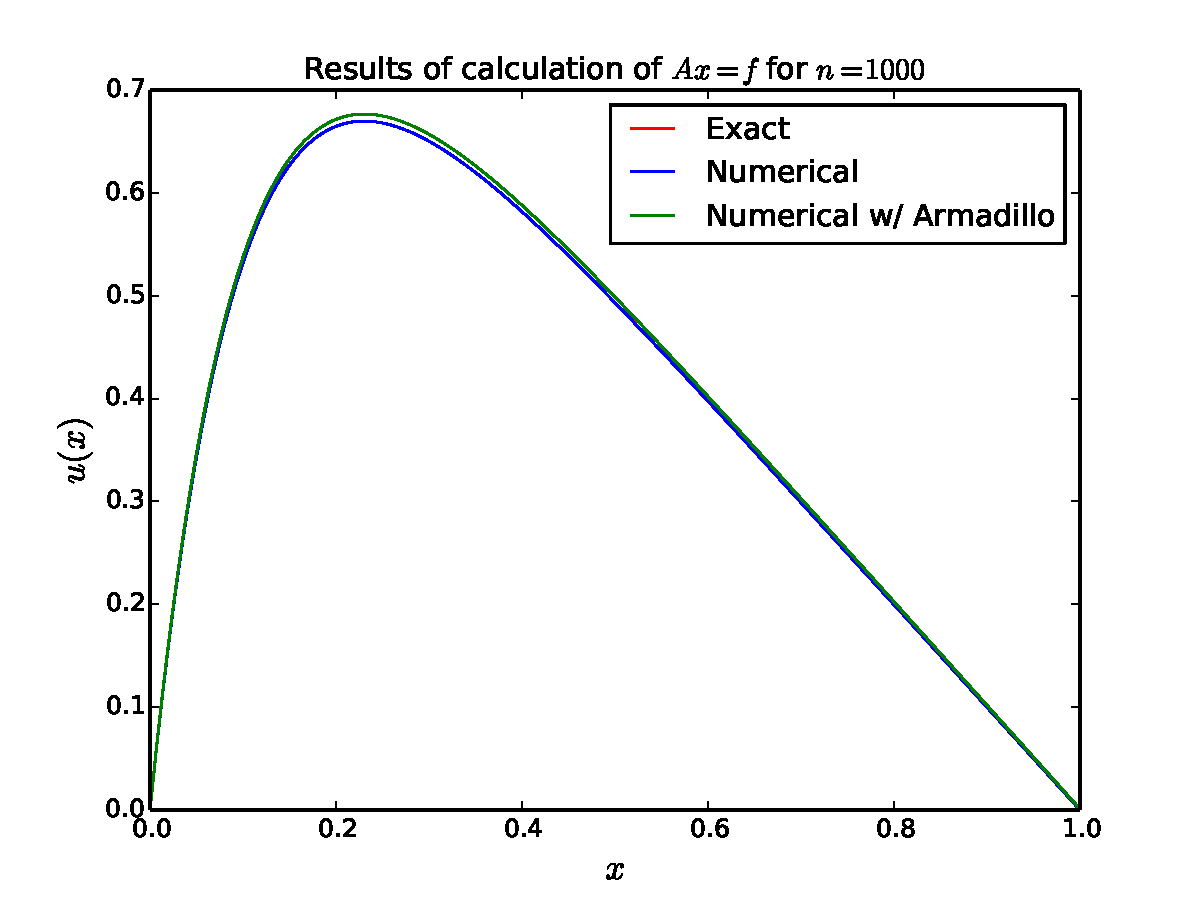
\includegraphics[width = .9\textwidth]{d_n_1000.pdf}
    \caption{Numerical solution for $n=10^5$.}
    \label{fig:sol103}
\end{figure}

\begin{figure}[H]
    \centering
    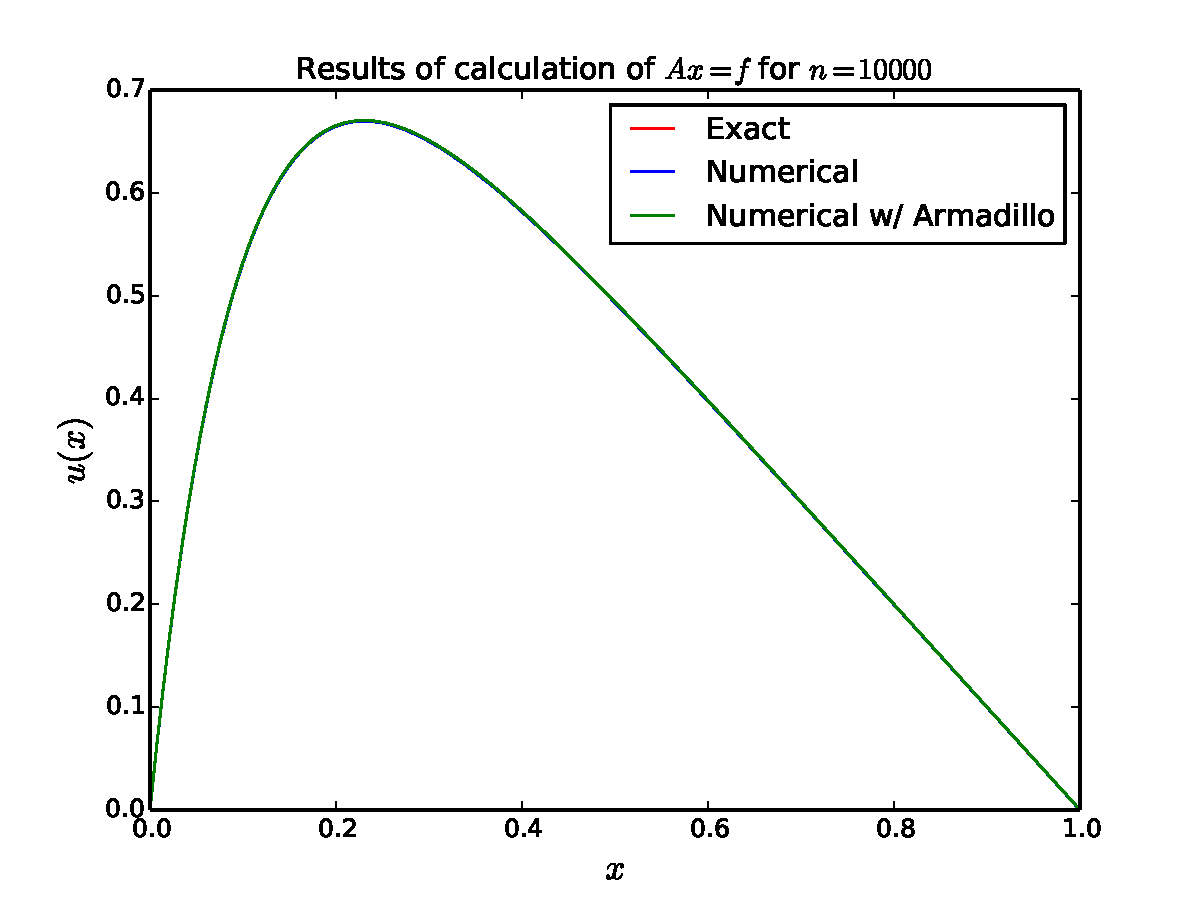
\includegraphics[width = .9\textwidth]{d_n_10000.pdf}
    \caption{Numerical solution for $n=10^5$.}
    \label{fig:sol104}
\end{figure}

\begin{table}[H]
  \centering
  \begin{tabular}{ c c c c }
    \toprule
    $n$ & $t_{\text{Numerical}}$ & $t_{\text{Armadillo}}$ & $t_{\text{LU decomp.}}$ \\
    \midrule
	$10$   & $0.000002$ s & $0.000075$ s & $0.000123$ s \\
	$10^2$ & $0.000004$ s & $0.000701$ s & $0.002931$ s \\
	$10^3$ & $0.000027$ s & $0.068193$ s & $0.459989$ s \\
	$10^4$ & $0.000312$ s & $40.02037$ s & $297.6299$ \\
    \bottomrule
  \end{tabular}
  \caption{Time spent by the different methods used to solve our problem. Something weird happens with the time-function when we set $n=10^4$ cause it didn't take five minutes to run the program on my own computer.}
  \label{tab:time}
\end{table}

When I'm setting $n=10^6$ Armadillo won't even make matrices for me, it tells me to use some other compilator, this may be because the matrices are too big for the ``normal'' Armadillo-library to handle when it comes to memory capacity.

\lstinputlisting[language=C++]{../arma_solve.cpp}
\lstinputlisting[language=C++]{../lu_decomposition.cpp}

Wikipedia says that LU-decomp. requires $(2/3)n^3$ FLOPS.

Armadillo won't compile when I'm trying to make $(10^6 \times 10^6)$-matrices.


\end{document}